\chapter{Studied Games and Known Results}
\label{ch:games}
We introduce a few examples of code-breaking games in this chapter.
The Counterfeit Coin problem and Mastermind game are quite well known,
  the other examples are based on various board games or less known
  logic puzzles.
We briefly summarize related research for each game, discuss
  its variations and applications and give a list of
  references.

Our goal in this work is neither to answer the research questions, nor
  to study possible generalizations.
We aim to create a general formalism and a computer language which could
  be used to describe arbitrary code-breaking game, if possible.
This chapter provides an overview of what we had in mind
  when we designed the framework and the language described
  in the rest of the thesis.

%%%%%%%%%%%%%%%%%%%%%%%%%%%%%%%%%%%%%%%%%%%%%%%%%%%%%%%%%%%%%%%%%%%%%%%%%%%%%%%%
\section{The Counterfeit Coin} \label{s:coins}

\begin{wrapfigure}{r}{0.26\textwidth}
  \begin{center}
  \vspace{-5mm}
  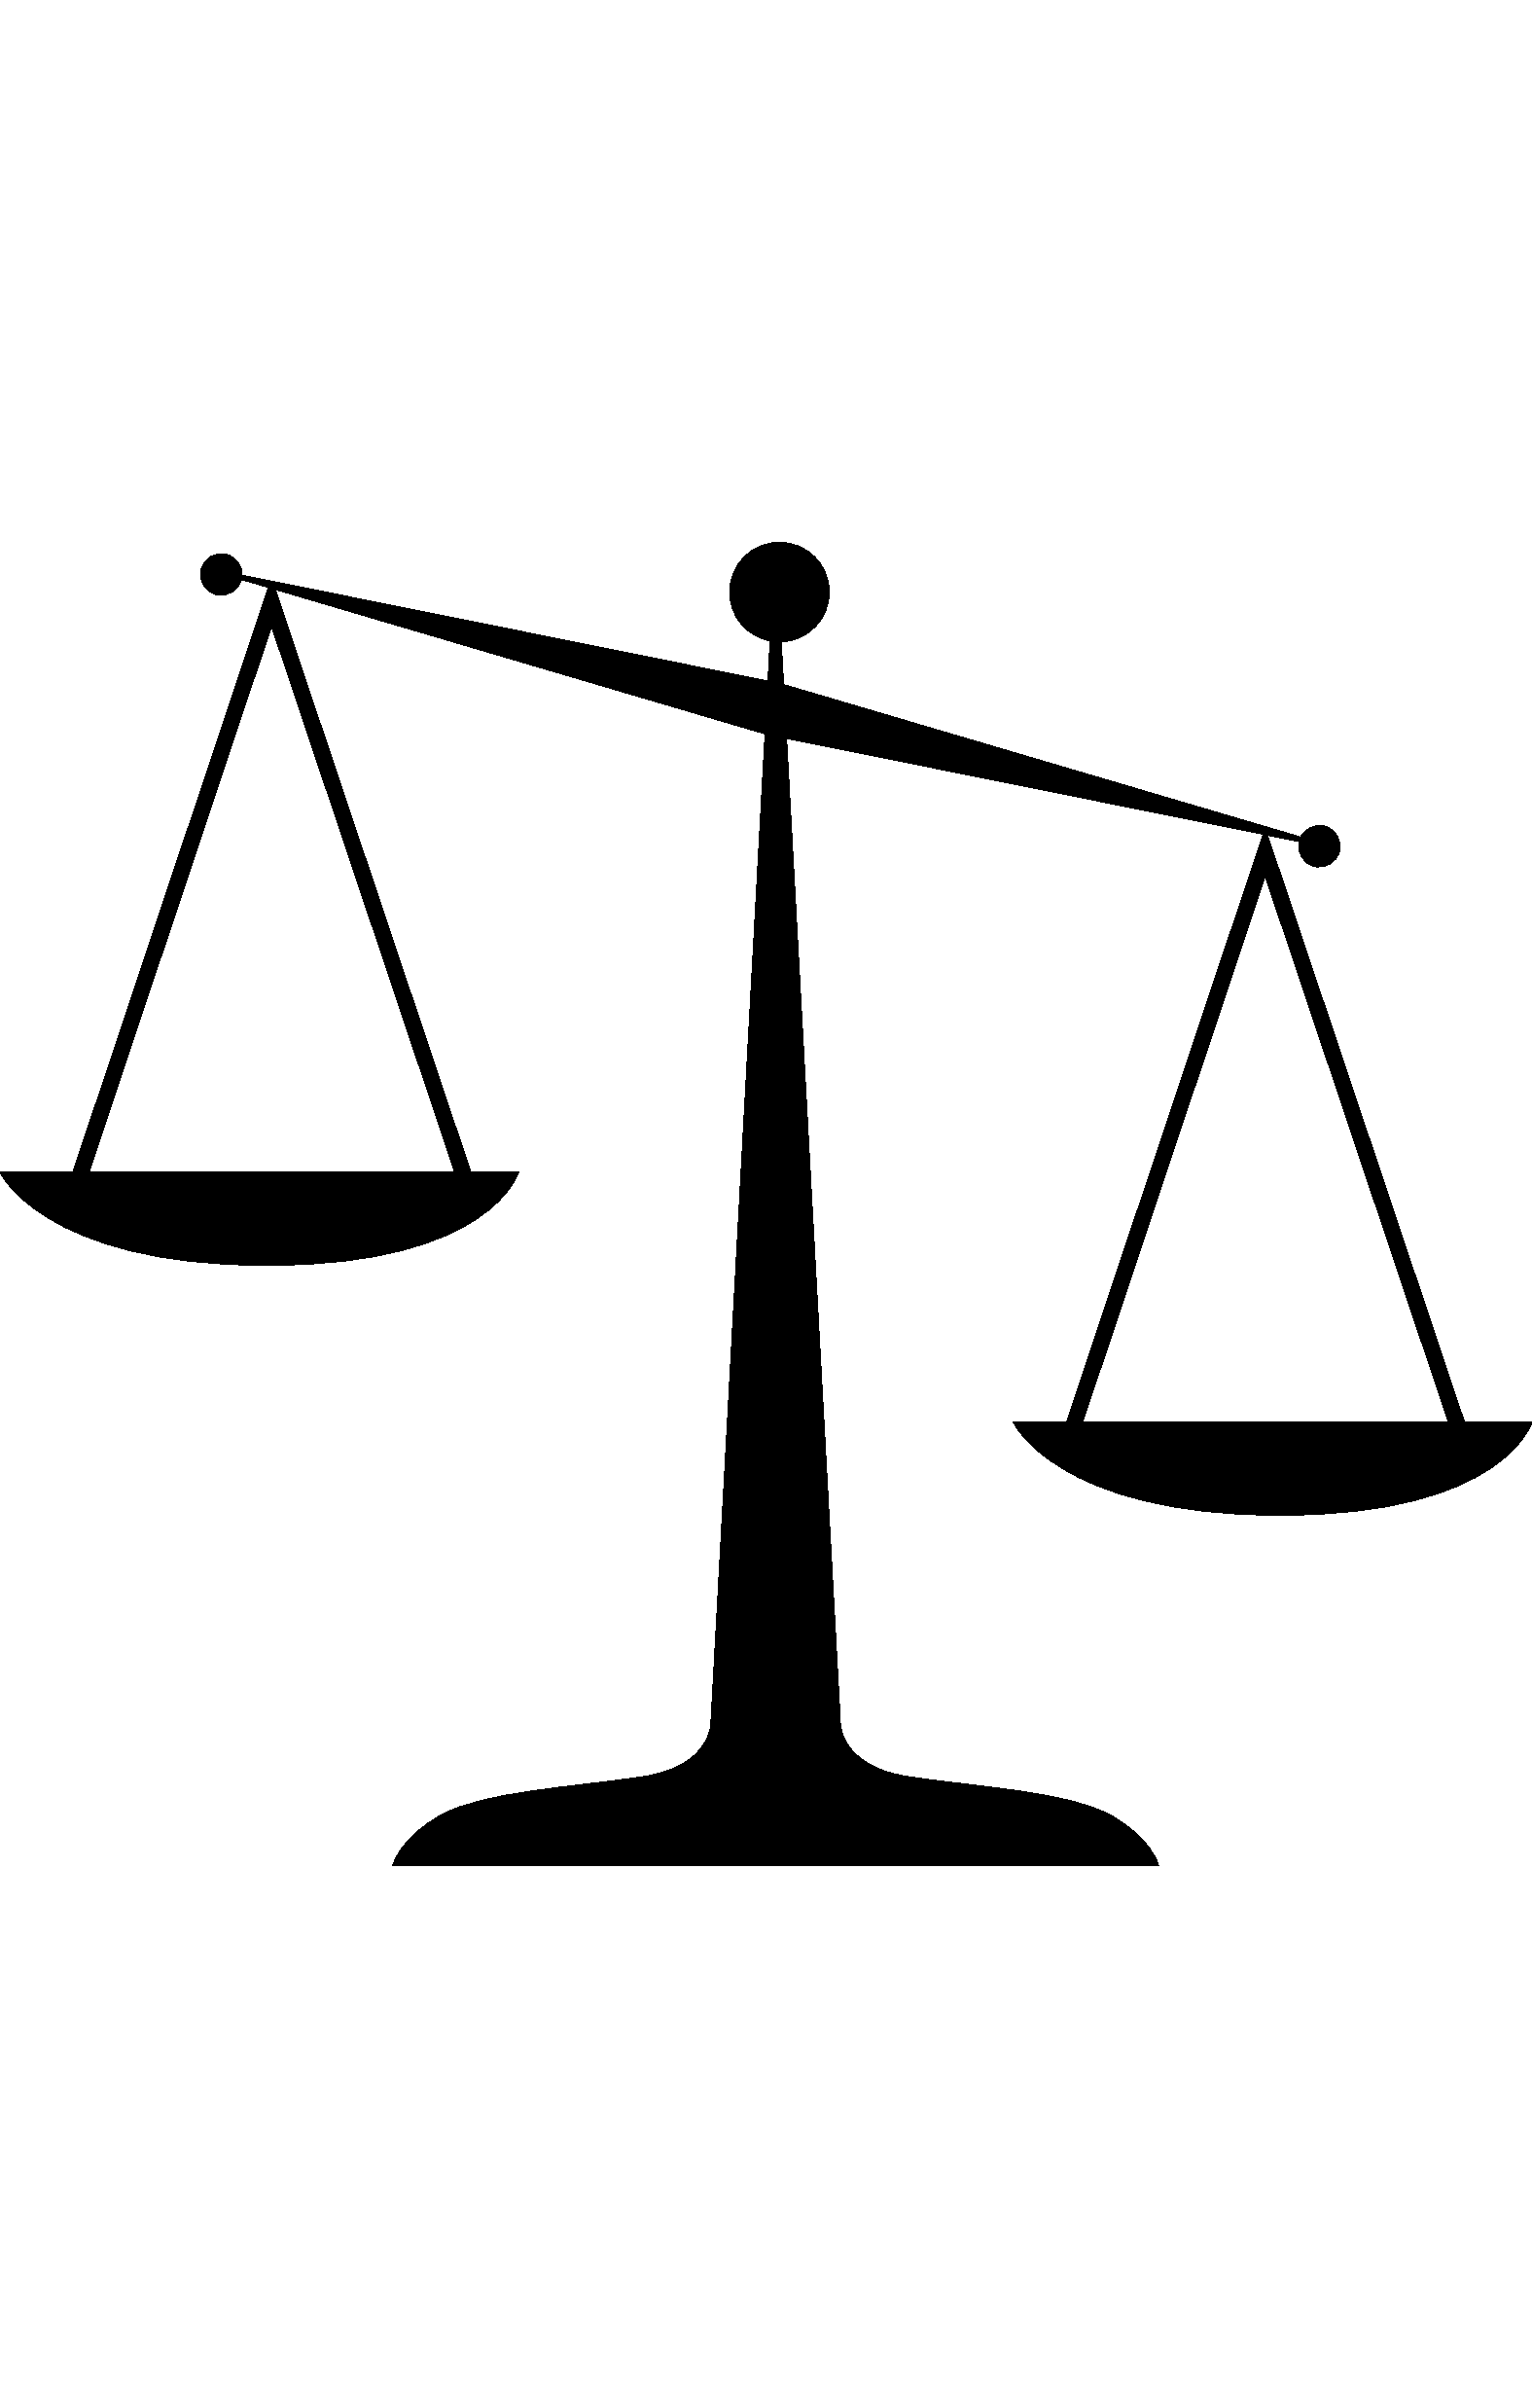
\includegraphics[width=0.23\textwidth]{pictures/scales.pdf}
  \vspace{-5mm}
  \end{center}
  \caption{Balance scale (illustrative image)\protect\footnotemark.}
  \vspace{-10mm}
\end{wrapfigure}
\footnotetext{Image adopted from
  \url{http://pixabay.com/en/justice-silhouette-scales-law-147214},
  under CC0 1.0 License.}

The problem of finding a counterfeit coin among regular coins in the fewest
  number of weighings on a balance scale is a folklore of
  recreational mathematics.

In all problems of this kind, you can only use the scale to weigh the coins.
You put some coins on the left pan, the same number of coins on the right pan
  and get one of the 3 possible outcomes.
Either both the sides weigh the same (denoted ``='')
  or the left side is lighter (``$<$''),
  or the right side is lighter (``$>$'').
The standard, easiest version can be formulated as follows.

\begin{problem}[The nine coin problem] \label{pr:coins9}
You are given $n >= 3$ (typically 9) coins, all except one having the same weight.
The counterfeit coin is known to be lighter.
Identify the counterfeit coin in minimal number of weighings.
\end{problem}

This problem is very easy as one can use \emph{ternary search} algorithm.
In short, we divide the coins into thirds, put one third against another
  on the scale.
If both pans weigh the same, the counterfeit coin must be in the last third,
  otherwise it must be on the lighter pan.
In this way, the size of the search space is reduced
  by a factor of 3 in each step, which is optimal.

In 1940s, more complicated version was introduced by Grossman\cite{coins-grossman1945}.

%whether the counterfeit coin is underweight or overweight
\begin{problem}[The twelve coin problem] \label{pr:coins12}
You are given $n >= 3$ (typically 12) coins, all except one having the same weight.
It is not known whether the counterfeit coin is heavier or lighter.
Identify the counterfeit coin and its weight relative to others
  in minimal number of weighings.
\end{problem}

The optimal solution for $n=12$ requires 3 weighings.
One of the optimal
  strategies is shown in \autoref{fig:coins12tree} as a decision tree.

\begin{figure}[h]
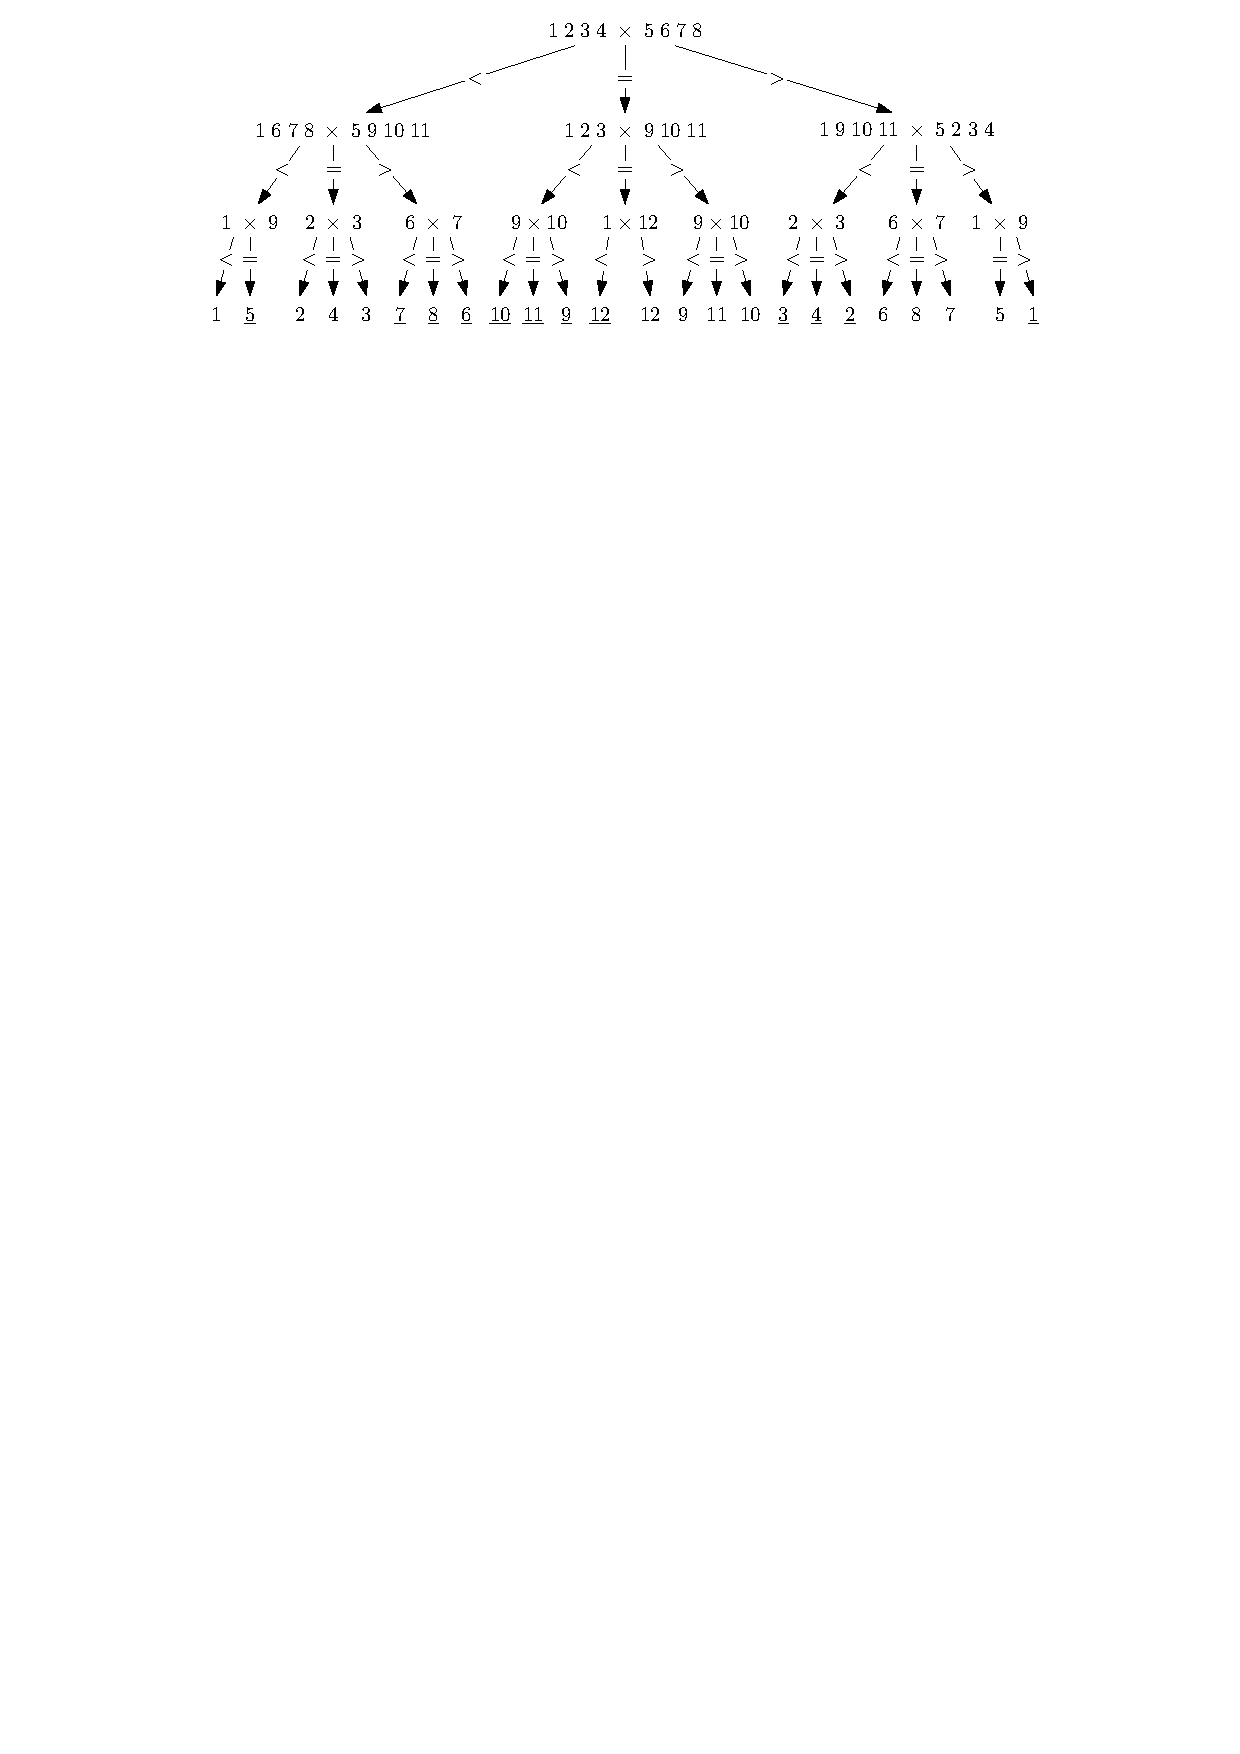
\includegraphics[width=\textwidth]{pictures/coins12.pdf}
\caption{Decision tree for The Twelve Coin Problem. \\
Leaf $x$ means that the coin number $x$ is lighter, $\underline{x}$ means that
the coin number $x$ is heavier.}
\label{fig:coins12tree}
\end{figure}

\subsection{Known results}

The research usually focuses on bounds on the maximal value of $n$
  for which the problem can be solved in $w$ weighings, for a given $w$.
Thus a solution of a problem is usually formulated as a theorem like the
  following one.

\begin{theorem}[Dyson, \cite{coins-dyson1946}]\label{th:coins12}
There exists a strategy that identifies the counterfeit coin and
  its type as described in \autoref{pr:coins12} with $w$ weighings,
  if and only if
  \[ 3 <= n <=\frac{3^w - 3}{2}. \]
\end{theorem}

\begin{proof}
We show the main part of the original Dyson's proof\cite{coins-dyson1946}
  here because of its elegant combinatorial idea.
We show a scheme for $n = \frac{1}{2}(3^w - 3)$.

Let us number the coins from $1$ to $n$.
To a coin number $i$, we assign
  two labels from $\{0,1,2\}^w$ -- those corresponding to the numbers
  $i$ and $3^w - 1 - i$ in ternary form.
Notice that all possible labels are used exactly once, except for $0^w, 1^w$
  and $2^w$, which were not assigned to any coin.
The labelling has the property that you can
  get one label of a coin from another by substituting $0$ by $2$ and $2$ by $0$.

A label is called ``clockwise'' if the first change of digit in it is
the change from $0$ to $1$, from $1$ to $2$, or from $2$ to $0$.
Otherwise, it is called ``anticlockwise''.
Thanks to the property we mentioned, one of the labels of a coin is always
  clockwise and the other is anticlockwise.

Let $C(i, d)$ be a set of coins such that $i$-th symbol in
  its clockwise label is $d$.
Since a permutation changing $0$ to $1$, $1$ to $2$ and $2$ to $0$ transfers
  coins from $C(i,0)$ to $C(i,1)$,
        from $C(i,1)$ to $C(i,2)$ and
        from $C(i,2)$ to $C(i,0)$,
  all the sets $C(i, d)$ contain exactly $n/3$ coins.
Now, let $i$-th experiment be the weighing of the coins $C(i,0)$ against $C(i, 2)$.
It remains to show that the experiments uniquely determine the counterfeit coin.
Let $a_i$ be 0, 1, or 2 if the result of $i$-th experiment is
  left side is lighter, both are the same, or right side is lighter, respectively.

If the counterfeit code is overweight, the $i$-th symbol of its clockwise label
  must be $a_i$. On the other hand, if it is underweight, the $i$-th symbol of
  its anticlockwise label must be $a_i$.
The solution of the problem is therefore the coin with the label $a_1a_2...a_w$
  and is heavier than others if and only if this label is clockwise.
\autoref{fig:coins12scheme} shows an example of the construction for
  $n = 12 = \frac{1}{2}(3^3 - 3)$, clockwise labels printed in bold.

\begin{figure}[h]
\begin{center}
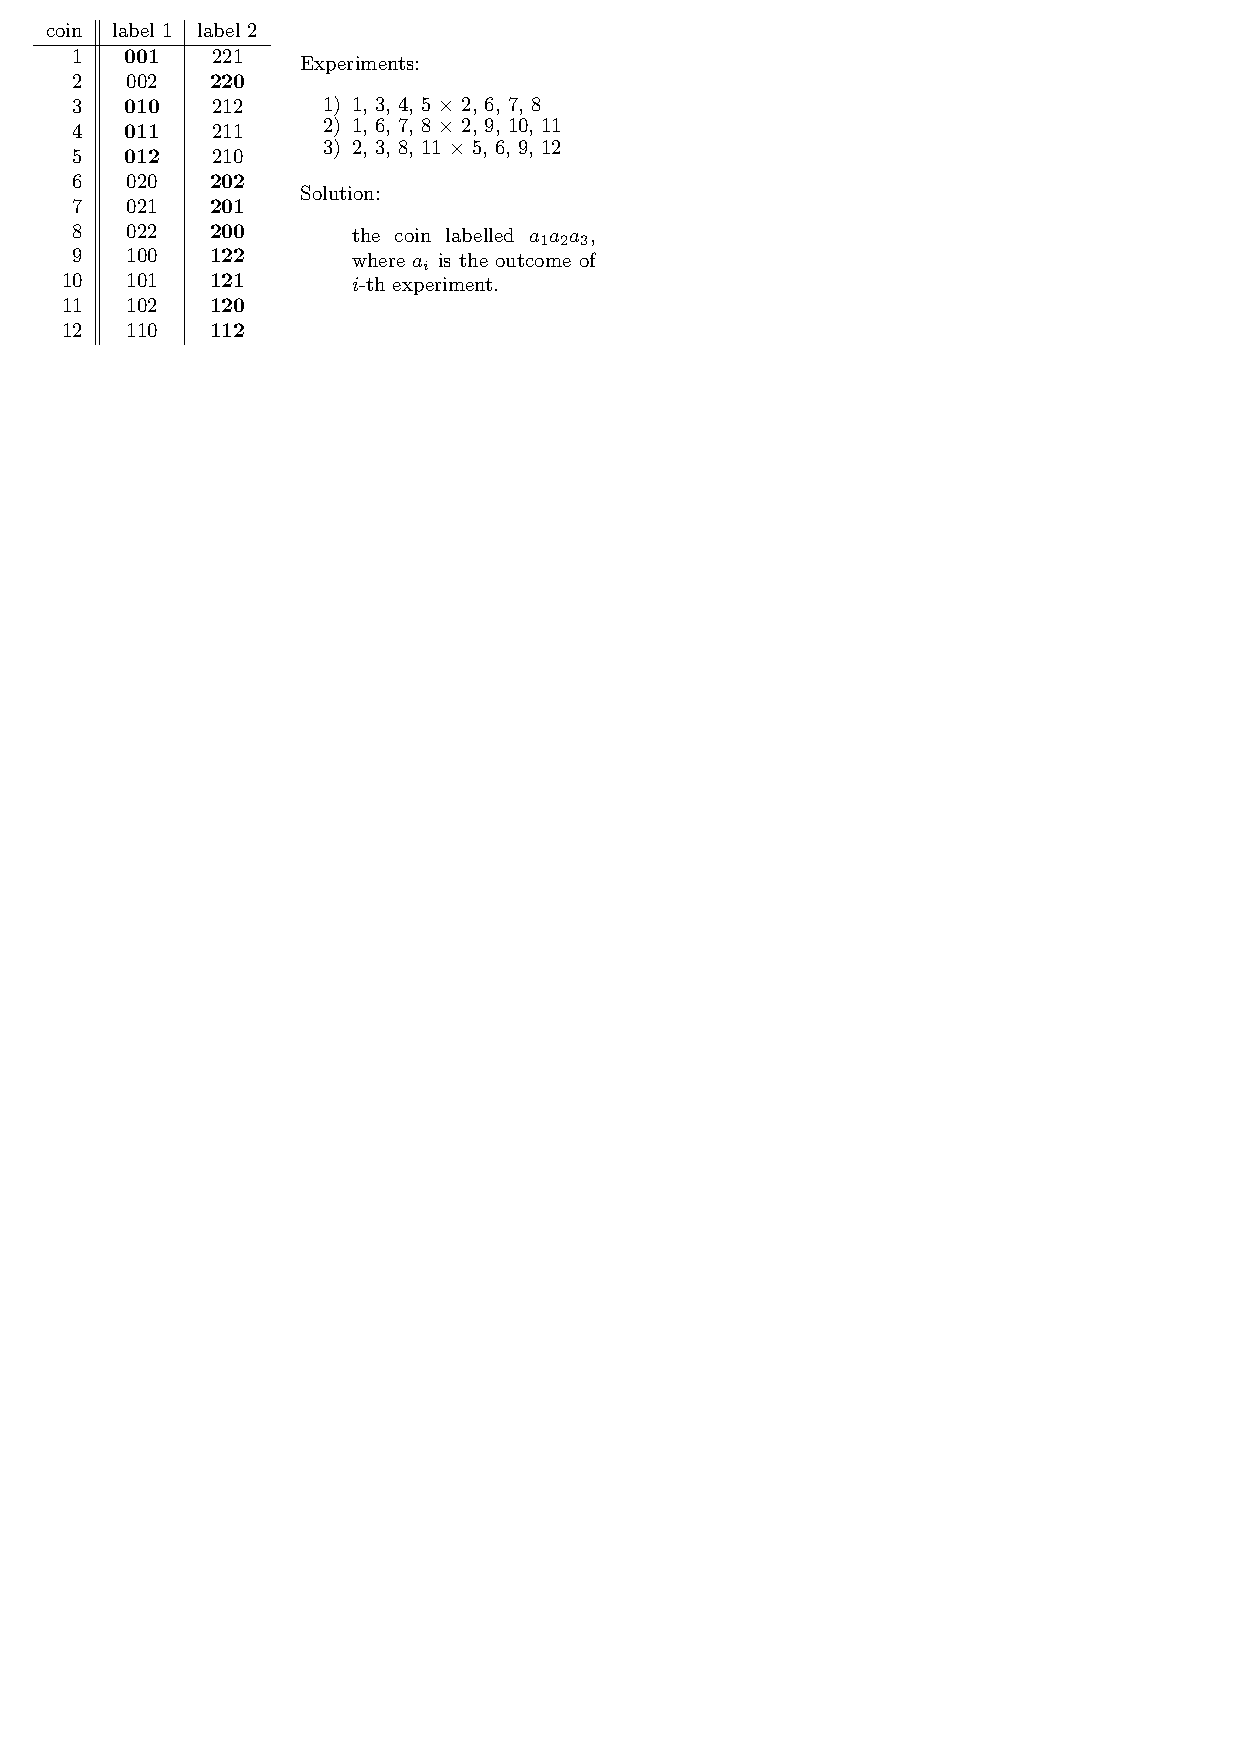
\includegraphics{pictures/coins12-th.pdf}
\end{center}
\caption{Demonstration of the ternary label construction for $n=12$.}
\label{fig:coins12scheme}
\end{figure}

The case $n < \frac{1}{2}(3^w - 3)$ can be solved similarly with some modifications
  to the labelling.
However, the scheme makes use of a genuine coin that was discovered in the first
  weighing and, therefore, the following experiments depend on the outcome of
  the first.
Finally, the proof that the coin cannot be identified for
  $n > \frac{1}{2}(3^w - 3)$ can be carried out using information theory.\qed
\end{proof}

\subsection{Generalizations and related research}

Naturally, the problem has been generalized in various ways and
  studied by many authors.
In ``Coin-Weighing Problems''\cite{coins-cwproblems1995}, Guy and Nowakovski
  gave a great overview of the research in the area until 1990s
  with an extensive list of references.
We list the most interesting variations and generalizations below.

\begin{description}
\item[Weight of counterfeit coin.]
  Either it is known whether the counterfeit coin is lighter or heavier,
  or it is not.
  The first one allows for more generalizations due to its simpler nature
  but both problems have been heavily researched.
\item[Number of counterfeit coins.]
  In the most common case, there is exactly one counterfeit coin,
    which allows for natural generalizations.
  First, a variation of \autoref{pr:coins9} with 2 or 3 counterfeit coins
   was studied\cite{coins-2fakes}\cite{coins-3fakes},
  then with $m$ counterfeit coins in general\cite{coins-mfakes}.
  Some authors studied the problem for unknown number of
  counterfeit coins\cite{coins-unknownfakes},
  or for \emph{at most} $m$ counterfeit coins\cite{coins-atmostfakes}.
\item[Additional regular coin(s).]
  In some cases, it may help if you are given an additional coin (or more coins),
    which is guaranteed not to be counterfeit.
  For example, for $n = 13$ in \autoref{pr:coins12}, you need 4 weighings.
  However, if you are given this one extra coin, you can determine the
    solution in just 3 weighings\cite{coins-dyson1946}.
\item[Non-adaptive strategies.]
  In this popular variation of the problem you have to announce all experiments
    in advance and then just collect the result.
  In other words, later weighings must not depend on the outcomes of the earlier weighings.
  Notice that the scheme constructed in the proof of \autoref{th:coins12} for
  $n = \frac{1}{2}(3^w - w)$ is indeed non-adaptive.
  However, the original proof uses an adaptive scheme for a smaller $n$.
  This was later updated, showing that there always exists an optimal scheme for
  \autoref{pr:coins12} which is non-adaptive\cite{coins-nonadaptive}.
\item[Unreliable balance.]
  This generalization introduces the possibility that
  one (or more) answers may be erroneous.
  The problem of errors/lies in general deductive games is well studied,
    see \cite{games-lies}.
  It was applied on the counterfeit coin problem (\autoref{pr:coins9} variant)
  in \cite{coins-unreliable} with at most one erroneous outcome or in
  \cite{coins-unreliable2} with two.
\item[Multi-pan balance scale.]
  In this variation, your balance scale has $k$ pans.
  You put the same number of coins on every pan and
    you get either the information that all
    weigh the same or which arm is lighter or heavier
    than others\cite{coins-multiplearm}.
\item[Parallel weighing.]
  In this generalization, you have 2 (or $k$, in general)
    balance scales, you can weigh different coins on
    the two scales simultaneously and it counts
    as one experiment only\cite{coins-parallel}.
  The motivation here is that weighing takes significant time,
  you have more scales and strive to minimize the time the whole process takes.
\end{description}

%%%%%%%%%%%%%%%%%%%%%%%%%%%%%%%%%%%%%%%%%%%%%%%%%%%%%%%%%%%%%%%%%%%%%%%%%%%%%%%%
\section{Mastermind}

\emph{Mastermind} is a classic code-breaking board game for 2 players,
  invented by Mordecai Meirowitz in 1970.
One player has the role of a \emph{codemaker} and the other of a \emph{codebreaker}.
First, the codemaker chooses a secret code of $n$ coloured pegs.
Then a codebreaker tries to reveal the code by making guesses.
The codemaker evaluates the guesses using black and white markers.
Black markers correspond to positions at which the code and the guess matches,
  a white marker means that some colour appears both in the code and in the guess,
  but at different positions.
The markers in the answer are not ordered, so the codebreaker does not know,
  which marker correspond to which peg in the guess.
Codebreaker's aim is to find out the code in minimal number of guesses.

More formally, let $C$ be a set of colours of size $c$.
Define a distance $d : C^n\times C^n -> \Nseto\times\Nseto$
  of two colour sequences by $d(u, v) = (b, w)$, where
\[
b = |\{ i \in\Nset \| u[i] = v[i] \}|
\]
\[
w = \sum_{j\in C} \min\big(\big|\{ i \| u[i] = j \}\big|,\;
                           \big|\{ i \| v[i] = j\}\big|\big)  - b.
\]
If the codemaker's secret code is $h$ and the codebreaker's guess is $g$,
  the guess should be evaluated with $b$ black pegs and $w$ white pegs, where
  $(b,w) = d(h,g)$.
Therefore, if the codebreaker have guessed $g_1, g_2, ..., g_k$ and the results
  were $(b_1,w_1), ..., (b_k, w_k)$,
  the search space is reduced to codes
  \[
  \{ u\in C^n \| \forall i<=k.\; d(u, g_i) = (b_i,w_i)\}.
  \]

\begin{wrapfigure}{r}{0.32\textwidth}
  \vspace{-5mm}
  \begin{center}
  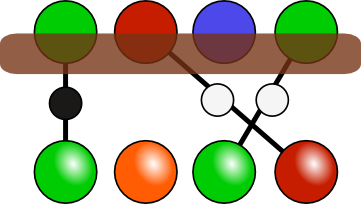
\includegraphics[width=0.25\textwidth]{pictures/mastermind-matching.png}
  \end{center}
  \caption{Guess evaluation by maximal matching.}
  \vspace{-5mm}
\end{wrapfigure}

Another way of looking at the guess evaluation is using
  \emph{maximal matching} of the pegs in the code $h$ and the guess $g$.
A matching is a set of pair-wise non-adjacent edges between
  pegs in the code (represented by $(0,i)$ for $1<=i<=n$) and
  pegs in the guess (represented by $(1,i)$ for $1<=i<=n$).
Let $M$ be a maximal matching such that

\begin{enumerate}
\item an edge connects only pegs of the same colour, i.e. if $((0,i),(1,i))\in M$, then $h[i] = g[j]$, and
\item if $h[i] = g[i]$ then $((0,i),(1,i))\in M$.
\end{enumerate}

Maximal means that no edge can be added without breaking one of the conditions.
The edges in $M$ correspond to the markers in the response,
  a marker being black if and only if the corresponding edge connects $(0,i)$
  with $(1,i)$ for some $i$.

\subsection{Known results and related research}

Much research has been done on this game, authors focusing
  on \emph{exact values}, \emph{asymptotics} (e.g. \cite{mm-chvatal}), or
  computer generated strategies.
One of the fundamental theoretical results is that
  \emph{Mastermind satisfiability problem}, asking
  whether there exists at least one valid solution,
  given a set of guesses and their scores, is NP-complete\cite{mm-np}.

When focusing on strategy synthesis, the goal is either to minimize
  \emph{the maximal number of guesses}
  or \emph{the expected number of guesses}, given that the code
  is selected from the set of possible codes with uniform distribution.
These two problems are quite different and strategies performing well
  in one case may perform poorly in the other.

Knuth\cite{mm-knuth} proposes a strategy that chooses a guess
  that minimizes the maximal number of remaining possibilities over all
  possible responses by the codemaker.
This strategy requires at most 5 guesses in the standard $n=4$, $c=6$ variant,
  which can be shown optimal.
In the average case, the strategy makes $4.48$ guesses.

Other authors proposed other \emph{one-step look-ahead} strategies.
Irving\cite{mm-expnum} suggested minimizing the expected number
  of remaining possibilities,
Neuwirth\cite{mm-entropy} maximized the entropy of the number
  of possibilities in the next round.
Much later, Kooi\cite{mm-mostparts} came up with a simple strategy that
  maximizes the number of possible responses by the codemaker,
  which is computationally easier and performs better that the previous two.

Using a backtracking algorithm, Koyama and Lai\cite{mm-exp-opt} found
  the optimal strategy for the expected case, which requires $4.34$
  guesses on average.
The comparison of the described strategies is shown in \autoref{tbl:one-step}.

\begin{table}[h]
\begin{center}
\begin{tabular}{|l|c|c|c|}
\hline Strategy & First guess & Expected-case & Worst-case \\ \hline
Maximal num. & AABB & 4.476 & 5 \\ \hline
Expected num. & AABC & 4.395 & 6 \\ \hline
Entropy & ABCD & 4.416 & 6 \\ \hline
Most parts & AABC & 4.373 & 6 \\ \hline
Exp-case optimal & AABC & 4.340 & 6 \\ \hline
\end{tabular}
\caption{Comparison of one-step look-ahead strategies. Data from \cite{mm-ville} and \cite{mm-mostparts}.}
\label{tbl:one-step}
\end{center}
\end{table}

Apart from \emph{one-step look-ahead} strategies, which are, in general,
  computationally intensive and do not scale well for bigger $n$ or $c$,
  other approaches has been suggested.
Many authors tried to apply genetic algorithms
  (see \cite{mm-ga} for an exhaustive overview and references therein),
  other analysed various heuristic methods (e.g. \cite{mm-heuristic}).

\subsection{Variations and applications}

\begin{description}
\item[Bulls and Cows]
is an old game with a principle very similar to Mastermind.
The only difference is that it uses digits instead of colours and does not allow repetitions.
Slovesnov wrote an exhaustive analysis of the problem, see \cite{bullsandcows}.


\item[Static mastermind] is a variation of the game in which all guesses
  must be made in one go.
The codebreaker prepares a set of guesses,
  then the codemakers evaluates all of them as usual and
  the codebreaker must determine the code from the outcomes.
This variation was introduced by Chvátal\cite{mm-chvatal} and
  partially solved (for $n<=4$) by Goddard\cite{mm-static},
  proving that for $4$ pegs and $k$ colours,
  the optimal strategy uses $k-1$ guesses.
Note that this corresponds to so-called \emph{non-adaptive} strategies
  for the Counterfeit Coin problem.

\item[String matching,] also called
  \emph{Mastermind with black-markers only}
  is a variation without white markers, i.e.
  you make guesses and the only information you get is the
  number of positions at which your guess is correct.
This problem was already studied by Erdős\cite{erdos-two}, who gave some
  asymptotic results about the worst-case number of guesses.
Later, this problem found an application in genetics with a need of
  methods to select a subset of genotyped individuals for phenotyping
  \cite{mm-app-gen2}\cite{mm-app-gen}.

\item[Extended Mastermind] was introduced by Focardi and Luccio,
  who showed that it is strictly related to cracking bank PINs for accessing ATMs
  by so-called \emph{decimalization attacks}\cite{mm-pins}.
In this variation, a guess is not just a sequence of colours, but a sequence of
  sets of colours. For example, if we have six colours $\{A, B, C, D, E, F\}$
  and the code is $AECA$,
  you can make a guess $\{A\}, \{C,D,E\}, \{A,B\}, \{F\}$, which
  will be awarded two black markers (for the first two positions)
  and one white marker (for $A$ guessed at position 3).
\end{description}

%%%%%%%%%%%%%%%%%%%%%%%%%%%%%%%%%%%%%%%%%%%%%%%%%%%%%%%%%%%%%%%%%%%%%%%%%%%%%%%%
\section{Other Problems}
\subsection{Black Box}

Black Box is a code-breaking board game in which one player creates a
  puzzle by placing four marbles on a $8\times 8$ grid.
The other player's goal is to discover their positions
  by the use of ``rays''.
The codebreaker chooses a side of the grid and an exact row/column, in which
  the ray enters the grid (thus having 32 choices).
For each ray, the codemaker announces the position, where the ray emerged from the grid,
  or says ``hit'', if the ray directly hit a marble\cite{blackbox}.

The marbles interact with rays in three ways:
\begin{description}
\item[Hit.] If a ray fired into the grid directly strikes a marble,
  the result is ``hit'' and the ray does not emerge from the box.
\item[Deflection.] If a ray does not directly strike a marble,
  but it should pass to one side of a marble, the ray is
  ``deflected'' and changes its direction by 90 degrees.
\item[Reflection.] If a ray should enter a cell with marbles on both sides,
  than it is ``reflected'' and returns back the same way it came.
  The same happens if a marble is at the edge of the grid
  and a ray is fired from a position next to it (so that it should be deflected
  even before entering the box according to the second rule).
\end{description}

\begin{figure}[h]
\begin{center}
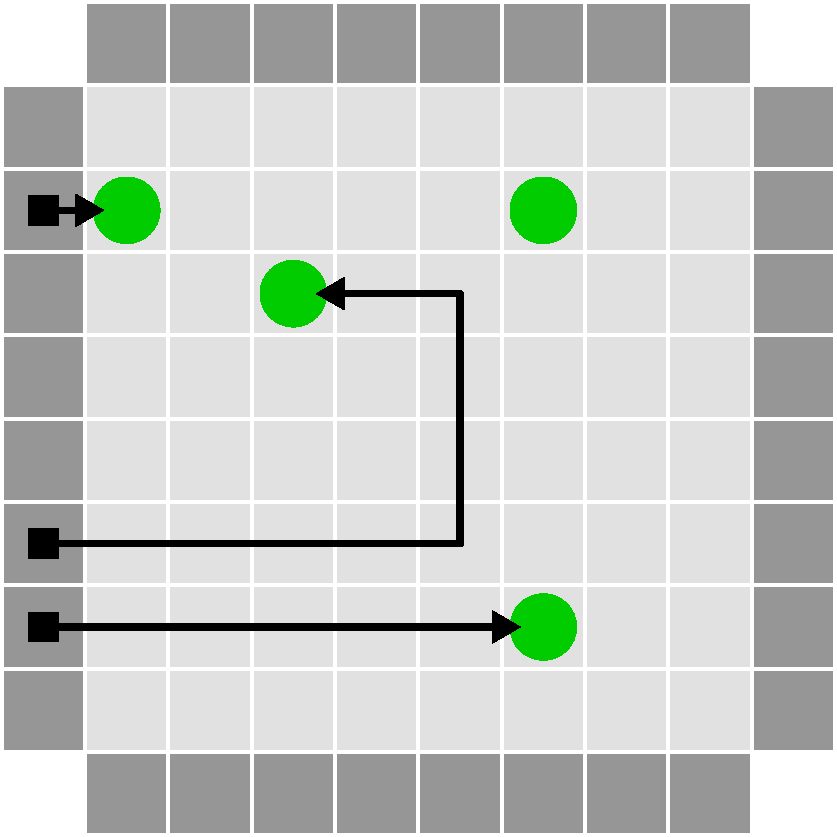
\includegraphics[width=.3\textwidth]{pictures/blackbox2.pdf} ~
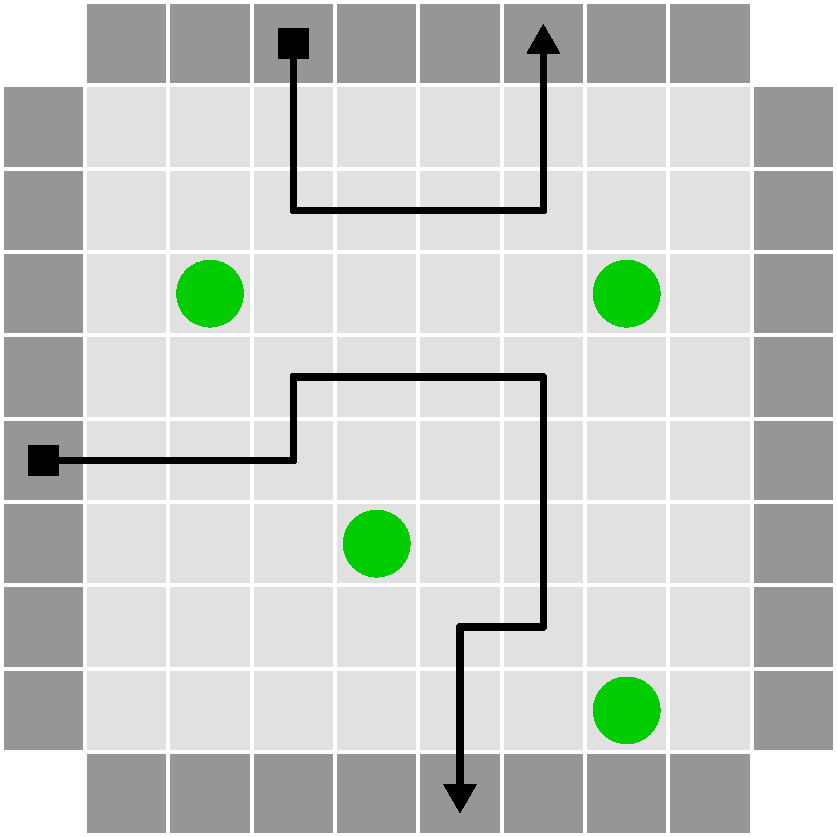
\includegraphics[width=.3\textwidth]{pictures/blackbox1.pdf} ~
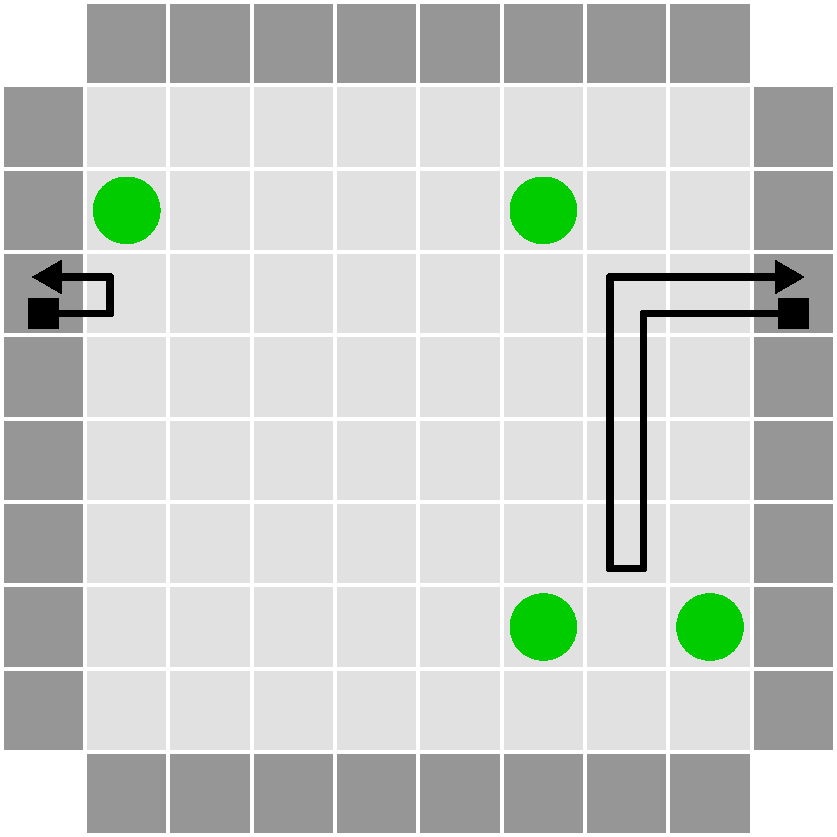
\includegraphics[width=.3\textwidth]{pictures/blackbox3.pdf} ~
\end{center}
\caption{Illustration of the rules of Black Box game\protect\footnotemark.}
\label{fig:blackbox-rules}
\end{figure}

\addtocounter{footnote}{-1}
\begin{wrapfigure}{r}{0.35\textwidth}
  \vspace{-10mm}
  \begin{center}
  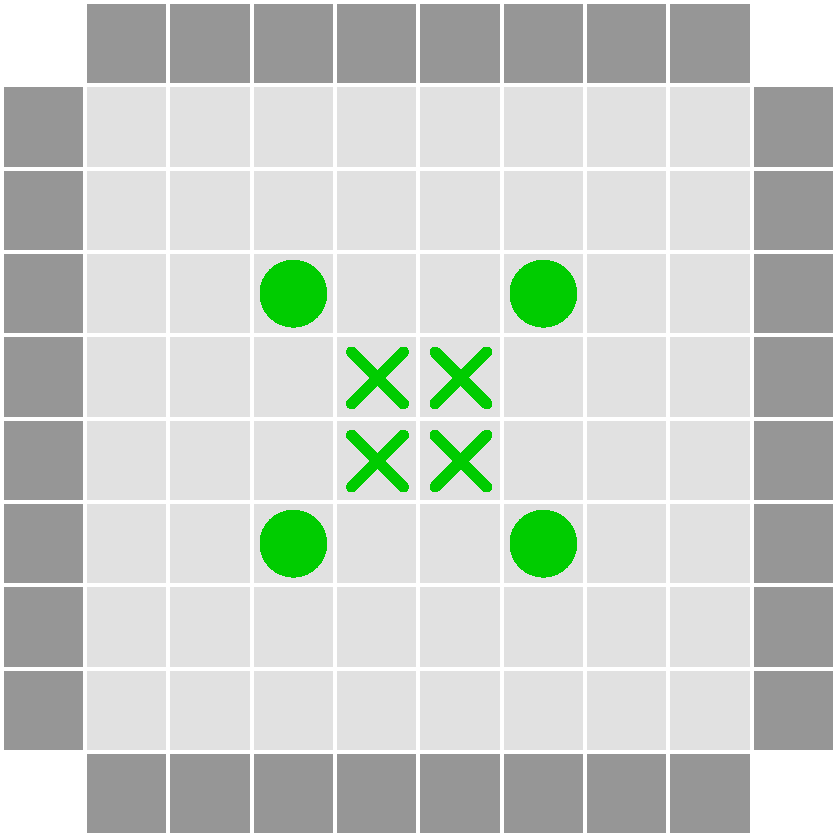
\includegraphics[width=0.3\textwidth]{pictures/blackbox-a.pdf}
  \end{center}
  \caption{An example of ambigous configuration\protect\footnotemark.}
  \label{fig:blackbox-ambigous}
\end{wrapfigure}

\footnotetext{Images adopted from \url{http://en.wikipedia.org/wiki/Black\_Box\_(game)} under GFDL 1.2. with minor modifications.}

A few examples are shown in \autoref{fig:blackbox-rules}.
The first image shows cases in which the ray hits the marble,
  the second shows rays deflected multiple times, emerging from
  the box at a different place, and the third demonstrates
  the two cases in which reflection happens.

Note that if the game is played with 5 or more marbles,
  they can be placed in the grid so that their position can
  not be uniquely determined.
\autoref{fig:blackbox-ambigous} shows an example of such
  problematic configuration.

Although Black Box is an interesting example of a code breaking game,
  there are configurations for which the codebreaker has to fire a ray from
  all positions to discover the marbles
  (and, for $5$ or more marbles, it may even be impossible),
  which makes the game uninteresting from a research point of view.

However, the game has become a popular puzzle for children and
  its principle has been used in other board games such as \emph{Laser maze}\cite{lasermaze}.

\subsection{Code 777}

During the board game named \emph{Code 777}, players sit in a circle,
  each drawing three cards at the beginning.
Players must not look at their own cards but they put them to a rack in front of them
  so that other players can see them.
Each card has one of seven colours and contains a number from one to seven.
The goal of the game is to determine which cards you have, using questions like
 ``Do you see more yellow sevens or blue fives?'', which the others answer\cite{code777}.

We can reformulate this as a code-breaking game, in which a player
  receives some cards, each having several attributes, each of which can have
  multiple values.
A player's goal is to determine his cards using questions
  like ``Do I have more [A] or [B]'', where [A] and [B] are conditions on
  any subset of attributes.
For example, if the attributes are number, colour, and shape, one can ask
  ``Do I have more triangles or green twos?''.

\subsection{Bags of Gold}

Imagine you have 10 bags of gold coins and
  you know that all coins in one bag are the same.
You were tipped off that some of the bags may contain counterfeit coins,
  which weigh 9 grams instead of 10 but are indistinguishable otherwise.
Suppose all coins in one bag are the same.
You have a digital scale that can show you exact weight of a set of coins.
How to find out which bags contain counterfeit coin in
  the minimal number of weighings?
Suppose there is a sufficient number of coins in each bag.

In the original version of this riddle, the scale has unlimited capacity and
  there is only one bag of counterfeit coins.
In that case, the secret can be determined in a single experiment.
You take one coin from the first bag, two coins from the second and so on up to
  10 coins from the last.
You put all those 55 coins on the scale and, if they are all good,
  they weigh 550 grams.
If the weight is by $x$ grams lower, you know that there are $x$ counterfeit
  coins in your set and, therefore,
  the $x$-th bag is the one with counterfeit coins.

The game gets more interesting if the capacity of the scale is limited, or
  if we have more bags and the number of coins in them is limited.
A special case, in which each bag contains a single coin is
  studied in \cite{erdos-two}, and is shown to be similar to the
  string matching problem (Mastermind with black-markers only).
Otherwise, the game lives only in a form of a logic puzzle and,
  to the best of our knowledge, no general results have been found.
